\section{The dip test and two limit laws}\label{sec:setting}

This section sets up the objects the rest of the paper compares: the dip, the uniform critical values, the limit law that the uniform calibration is built on, and the limit law that replaces it on a flat shoulder.

\subsection{The dip}
A distribution function $F$ is \emph{unimodal} if, for some point $m$, it is convex to the left of $m$ and concave to the right. Equivalently, its density rises up to $m$ and falls after it. Flat stretches are allowed, and so is a modal interval instead of a single mode. This is the definition of Hartigan and Hartigan \cite{HH85}, and we use it throughout. We call $F$ \emph{continuous unimodal} if in addition it has no atom.

The dip of a distribution function $G$ is its largest vertical distance to the nearest unimodal distribution function. For a sample $X_1,\dots,X_n$ with empirical distribution function $F_n$, the dip statistic is $D_n=D(F_n)$. The dip does not change under an increasing affine change of variable, so we may put the data in $[0,1]$. Hartigan and Hartigan \cite[Theorem~1]{HH85} also showed that the constraint ``is a distribution function'' can be dropped: for $G$ on $[0,1]$, $D(G)$ equals the distance from $G$ to the bounded functions that are convex on $[0,m]$ and concave on $[m,1]$ for some $m$. We call $m$ the \emph{turning point} of such a function. This form lets us take the dip of any bounded function $h$, which we need because the limits below are dips of random continuous functions.

The argument uses a one-sided version of the dip, the distance to the nearest convex function. The \emph{convex distance} of a bounded function $h$ on an interval $I$ is
\[
V_I(h)=\inf\Bigl\{\sup_{x\in I}|h(x)-g(x)| : g \text{ convex on } I\Bigr\},
\]
and we write $V(h)$ when $I=[0,1]$. The \emph{concave distance} $C_I(h)$ is defined in the same way with concave functions in place of convex ones. A convex function is a unimodal fit whose turning point sits at the right end, so $D(h)\le V(h)$ always. The dip can choose its turning point and the convex distance cannot. \Cref{sec:mechanism} shows that a flat shoulder takes this choice away.

\subsection{The uniform calibration}
Under the uniform law on $[0,1]$ the distribution of $D_n$ depends only on $n$. Let $q_n(1-\alpha)$ be its $(1-\alpha)$ quantile. The \emph{standard test} at level $\alpha$ rejects unimodality when $D_n\ge q_n(1-\alpha)$. We always mean the exact uniform quantile here, so simulation error in published tables plays no role.

Hartigan and Hartigan proved that under the uniform law $\sqrt nD_n$ converges in distribution to $D(B)$, the dip of a standard Brownian bridge $B$ \cite[Theorem~3]{HH85}. Let $\qbar_\alpha$ be the $(1-\alpha)$ quantile of $D(B)$. If the distribution function of $D(B)$ has neither a jump nor a flat stretch at $\qbar_\alpha$, the scaled critical values converge, $\sqrt n\,q_n(1-\alpha)\to\qbar_\alpha$. This condition is not proved, but every simulation we ran supports it, and we assume it wherever a result is stated in terms of $\qbar_\alpha$. Roughly, $\qbar_{0.05}\approx0.546$ and $\qbar_{0.01}\approx0.63$; certified ranges follow in \cref{sec:numbers}.

\subsection{The concave-majorant gap}
The second limit law comes from a different functional of the bridge. Let $\LCM(B)$ be the least concave majorant of $B$ on $[0,1]$, the smallest concave function lying above it, and let
\[
M=\sup_{0\le u\le1}\bigl(\LCM(B)(u)-B(u)\bigr)
\]
be the largest vertical gap between the two. Balabdaoui and Pitman \cite{BP11} found the law of $M$; it has a density and mean about $0.9994$. Balabdaoui and Filali \cite{BF11} tabulated its distribution function, which we write $F_M$. Since $-B$ is again a Brownian bridge, the largest gap between $B$ and its greatest convex minorant also has the law of $M$; this is the form in which $M$ appears in \cref{sec:mechanism}. We define
\[
c_\alpha=\tfrac12F_M^{-1}(1-\alpha),
\]
so that $P(M/2>c_\alpha)=\alpha$. Its values are $c_{0.10}\approx0.668$, $c_{0.05}\approx0.7314$ and $c_{0.01}\approx0.8599$. \Cref{fig:limits} compares the two limit laws. At the uniform 5 percent cutoff $\qbar_{0.05}$, the law of $M/2$ still has about 30 percent of its mass to the right.

\begin{figure}[t]
\centering
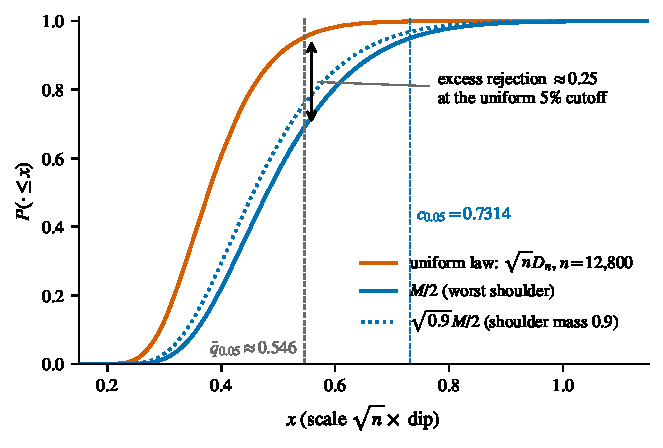
\includegraphics[width=0.78\linewidth]{figs/fig2_limit_laws.pdf}
\caption{At the uniform 5 percent cutoff, the shoulder limit $M/2$ still puts about 30 percent of its mass above the cutoff, while the uniform limit puts 5 percent there. Orange: the distribution function of $\sqrt nD_n$ under the uniform law, from $10^5$ simulated samples at $n=12{,}800$; its 95 percent point is close to $\qbar_{0.05}\approx0.546$. Solid blue: the distribution function of $M/2$, from the table of Balabdaoui and Filali. Dotted blue: $\sqrt{0.9}\,M/2$, the shoulder term for a shoulder of mass 0.9; for the running example the full limit is the larger of this term and an independent term $\sqrt{0.1}\,D(B')$ from the top, which hardly ever matters at these cutoffs (\cref{sec:mechanism}). The vertical distance between the curves at $\qbar_{0.05}$ is the excess rejection rate that a shoulder of nearly full mass produces. The constant $c_{0.05}=0.7314$ is the 95 percent point of $M/2$.}
\label{fig:limits}
\end{figure}

\subsection{Limiting rates and worst cases}
Rejection probabilities need not converge, and we never need them to. When we say that a limiting rejection rate is at most $x$, we mean that its limit superior is at most $x$; when we say it is at least $x$, we mean its limit inferior.

Two questions about the null hypothesis sound alike but are different. The first fixes a law $F$, lets $n$ grow, and then asks for the worst law; this is the \emph{pointwise} question, answered in \cref{sec:mechanism,sec:size}. The second fixes $n$, takes the worst law at that $n$,
\[
S_n(\alpha)=\sup_{F\ \text{continuous unimodal}}P_F\bigl(D_n\ge q_n(1-\alpha)\bigr),
\]
and then lets $n$ grow; this is the \emph{worst-case size} $S_n(\alpha)$, the quantity a user who does not know the law actually faces. It is at least as large as the pointwise answer, because a law that changes with $n$ is allowed. \Cref{sec:worst} shows that, for the dip, both answers lie in the same interval.

For the pointwise results we need a class of laws regular enough to analyse. Let $\cC$ be the atomless unimodal laws on a bounded interval whose one-sided densities at the mode are finite. It contains every unimodal step density, trapezoids, the triangular law, Beta$(a,b)$ laws with $a,b>1$ and truncated normal laws. It excludes unbounded support, an infinite density at the mode and atoms.

\subsection{What the numbers guarantee}\label{sec:numbers}
Several constants in this paper are computed, and we use two kinds of guarantee for them.

A value is \emph{rigorously enclosed} when it is computed in ball arithmetic, which carries every rounding error into the result. We enclose $F_M$ on a fine grid with the Arb library \cite{Arb}, starting from the stick-breaking representation of Balabdaoui and Pitman with an explicit bound on the remainder of its series. This gives $c_{0.10}\in[0.667,0.6685]$, $c_{0.05}\in[0.7305,0.7325]$ and $c_{0.01}\in[0.8585,0.861]$. A finer floating-point enclosure, which pads the error but is not rigorous in the same sense, gives $c_{0.05}\in[0.7313,0.7315]$ and $c_{0.01}\in[0.8598,0.8599]$.

A value is \emph{certified} when it comes from a Monte Carlo computation whose code, random seeds, sample size and decision rule were fixed in a written protocol before it ran, and whose decision rule uses exact binomial or Bernstein bounds with a correction for every claim in the run. If the claimed statement were false, the run would certify it with probability at most a stated $\delta$. The probability refers to the random draws, not to the statement. In this way we bracket the limiting uniform critical values: from $12{,}000$ simulated bridges on a grid of $2\cdot10^6$ points, with lower and upper bounds on $D(B)$ for each path,
\[
\qbar_{0.05}\in[0.5379,\,0.5558],\qquad \qbar_{0.01}\in[0.6162,\,0.6438],
\]
jointly with confidence at least $0.99$, and $\qbar_{0.10}\in[0.4936,\,0.5108]$ with confidence at least $0.998$. The value $0.5452$ in the \texttt{diptest} table at $n=72{,}000$ lies inside the first bracket. Most of the width of the size intervals quoted later comes from these brackets.

\subsection{Related work}\label{sec:prior}
Besides the work cited in \cref{sec:intro}, three lines of research are close to ours. Müller and Sawitzki \cite{MS91} and Polonik \cite{Polonik95} developed the excess-mass approach to modality; in one dimension the excess-mass statistic for two modes equals twice the dip \cite{CH98}. Cheng and Hall \cite{CH98} replaced the uniform calibration by one fitted to the curvature at the mode, and in a second paper \cite{CH99} showed that a shoulder near the mode makes such calibrations anticonservative and proposed a shoulder-aware version. Their shoulders are smooth; ours are stretches of constant density that end in a jump. Davies and Kovac \cite{DK04} used a Kuiper-type distance, which gives a conservative cutoff for the dip that is valid at every $n$, and Hartigan \cite{Hartigan00} proposed a statistic aimed at shoulders and antimodes.

For the one-sided question, whether a distribution function is concave, the uniform \emph{is} least favourable. Kulikov and Lopuhaä \cite{KL08} proved this for the supremum distance to the least concave majorant, even at fixed $n$, Carolan \cite{Carolan02} obtained closely related results, and Beare \cite{Beare21} extended least favourability to $L^p$ distances in the limit. Carolan and Dykstra \cite{CD99} studied the Grenander estimator at flat regions of a density, a one-sided version of the effect that flat stretches have here. Beare and Fang \cite{BF17} computed the directional derivative of the least concave majorant at a distribution function with affine pieces, a tool we use. The one-sided results do not carry over to the dip because the dip lets its fit turn, and the turning point is exactly what a flat shoulder constrains.
